% Étape 0 : données.
% Sources : julia/, configs/base.yaml, notebooks/00_donnees.ipynb, results/etape0/, data/spx/.

\section{Données}
\label{sec-donnees}

Le réseau apprend la fonction qui associe aux cinq paramètres de Heston une surface de volatilité implicite.
Il faut donc un pricer de référence fiable, un jeu de surfaces simulées qui couvre le domaine utile, et des
surfaces de marché pour l'étape de calibration (\cref{sec-calibration}). Cette section les décrit et explique nos
choix.

\subsection{Le modèle et la grille}
\label{sec-modele}

On écrit le modèle de \citet{heston1993} directement sur le prix forward $F_t$ (taux nul, dividendes inclus dans
le forward), avec une variance instantanée $v_t$ qui revient vers sa moyenne :
\begin{equation}
  \frac{dF_t}{F_t} = \sqrt{v_t}\, dW_t, \qquad
  dv_t = \kappa(\theta - v_t)\, dt + \xi \sqrt{v_t}\, dZ_t, \qquad
  d\langle W, Z\rangle_t = \rho\, dt .
  \label{eq-heston}
\end{equation}
Les cinq paramètres sont la variance initiale $v_0$, la variance de long terme $\theta$, la vitesse de retour
$\kappa$, la volatilité de la variance $\xi$ et la corrélation $\rho$. Le ratio de \citet{feller1951}
$2\kappa\theta/\xi^2$ indique si la variance peut toucher zéro (ratio inférieur à 1) ; on y reviendra.

On normalise $F_0 = 1$ : le strike $K$ est alors directement la moneyness $K/F_0$. Une surface est l'ensemble des
volatilités implicites de Black-76 \citep{black1976} sur une grille fixe de
\num{8} maturités ($T \in \{0{,}1 ; 0{,}3 ; 0{,}6 ; 0{,}9 ; 1{,}2 ; 1{,}5 ; 1{,}8 ; 2\}$ ans) et
\num{11} strikes ($K$ de \num{0.5} à \num{1.5} par pas de \num{0.1}), soit \num{88} valeurs : c'est la sortie
du réseau. Les erreurs sont exprimées en points de base de volatilité ($1\pb = \num{0.01}$ point de vol,
par exemple \SI{20.00}{\percent} au lieu de \SI{20.01}{\percent}).

\subsection{Le pricer de référence}
\label{sec-pricer}

Le pricer est écrit en Julia (\texttt{julia/src/HestonFourier.jl}) pour la vitesse. Pour une maturité donnée, il
calcule les prix de toutes les options de la grille par la méthode COS de \citet{fang2008} : la densité du
log-rendement $x = \log(F_T/F_0)$ est développée en série de cosinus sur un intervalle $[a,b]$,
\begin{equation}
  f(x) \approx {\sum_{k=0}^{N-1}}' A_k \cos\!\Big(k\pi\frac{x-a}{b-a}\Big), \qquad
  A_k = \frac{2}{b-a}\, \mathrm{Re}\Big[\varphi\Big(\frac{k\pi}{b-a}\Big) e^{-ik\pi a/(b-a)}\Big],
\end{equation}
où $\varphi$ est la fonction caractéristique de Heston, écrite sous la forme « little Heston trap » de
\citet{albrecher2007} pour éviter les discontinuités du logarithme complexe. Les coefficients $A_k$ sont calculés
une seule fois par maturité ; chaque strike ne coûte ensuite qu'une somme. On price toujours l'option hors de la
monnaie (put si $K<1$, call sinon) : son prix est petit mais calculé directement, sans passer par la parité
call-put qui ferait perdre de la précision. Le nombre de termes part de $N = 256$ et double tant que
$|\varphi(N\pi/(b-a))| > 10^{-15}$. La volatilité implicite est obtenue en inversant la formule de Black-76 par la
méthode de Brent.

\paragraph{Trois corrections de précision.} En vérifiant le pricer contre une méthode indépendante (formule de
\citet{lewis2000}, intégration numérique), nous avons trouvé et corrigé trois défauts :
\begin{itemize}
  \item l'intervalle $[a,b]$ est centré sur la moyenne $c_1$ du log-rendement, avec une largeur proportionnelle à
  son écart-type $\sqrt{c_2}$. La formule fermée de $c_2$ que nous utilisions donnait une variance
  \emph{négative} pour environ \SI{20}{\percent} des paramètres tirés. Nous calculons désormais $c_1$ et $c_2$
  directement à partir de la fonction caractéristique ($\log\varphi(u) \approx i c_1 u - c_2 u^2/2$, par
  différences finies) ;
  \item un intervalle de $\pm 12$ écarts-types est trop étroit quand la condition de Feller est très violée : la
  queue gauche de la densité est alors épaisse, et l'erreur pouvait atteindre plusieurs centaines de points de
  base. Nous prenons $\pm 32$ écarts-types, avec une borne droite plafonnée à $b = 10$ (au-delà, le terme $e^{b}$
  du calcul des calls fait perdre de la précision, alors qu'un rendement de $e^{10}$ n'a aucune probabilité) ;
  \item en dessous d'un prix de $10^{-10}$, l'erreur numérique de la méthode (quelques $10^{-12}$) fausse la
  volatilité implicite de plusieurs points de base : ces points sont marqués comme manquants (NaN), au lieu du
  seuil de $10^{-12}$ utilisé au départ.
\end{itemize}
Après correction, l'écart maximal avec la formule de Lewis est de \SI{0.002}{\pb} sur près de \num{39000} points,
choisis au hasard et parmi les cas les plus difficiles (forte volatilité, maturité longue, condition de Feller très
violée). Le pricer est couvert par \num{274} tests automatiques : prix de référence publié par \citet{fang2008},
limite de Black-Scholes, absence d'arbitrage (prix des calls décroissants et convexes en $K$), et les cas
difficiles ci-dessus.

\paragraph{Une copie en Python.} Le même pricer existe en Python (module \texttt{heston\_cos}), pour vérifier
le code Julia et pouvoir calibrer sans Julia. Recalculées en Python à partir des mêmes paramètres,
les \num{50000} surfaces d'entraînement sont identiques : les NaN sont exactement aux mêmes endroits, et l'écart
est de \SI{1e-6}{\pb} en moyenne (\SI{0.07}{\pb} au maximum, sur des calls très loin de la monnaie dont le prix est
proche du seuil).

\subsection{Le domaine des paramètres}
\label{sec-plages}

Le réseau n'apprend que ce qu'on lui montre : le domaine de tirage des paramètres doit couvrir les surfaces qu'on
voudra calibrer, sans gaspiller des exemples sur des régimes irréalistes. Le \cref{tab-plages} donne notre choix
(\texttt{configs/base.yaml}).

\begin{table}[H]
  \centering
  \caption{Domaine de tirage des paramètres, comparé au code Heston de \citet{horvath2021}.}
  \label{tab-plages}
  \small
  \begin{tabular}{lccl}
    \toprule
    Paramètre & Notre domaine & \citet{horvath2021} & Commentaire \\
    \midrule
    $v_0$      & $[0{,}0049 ; 0{,}16]$ & $[0{,}0001 ; 0{,}04]$ & vol initiale de \SI{7}{\percent} à \SI{40}{\percent} \\
    $\theta$   & $[0{,}01 ; 0{,}16]$   & $[0{,}01 ; 0{,}20]$   & vol de long terme de \SI{10}{\percent} à \SI{40}{\percent} \\
    $\kappa$   & $[0{,}5 ; 10]$        & $[1 ; 10]$            & \\
    $\xi$      & $[0{,}1 ; 1{,}5]$     & $[0{,}01 ; 1]$        & souvent supérieur à 1 sur le SPX \\
    $\rho$     & $[-0{,}95 ; -0{,}1]$  & $[-0{,}95 ; -0{,}1]$  & toujours nettement négatif sur le SPX \\
    Feller     & $2\kappa\theta/\xi^2 \geq 0{,}1$ & $\geq 1$ pour tout leur jeu & \\
    \bottomrule
  \end{tabular}
\end{table}

L'article de \citet{horvath2021} ne donne pas de domaine pour Heston ; les valeurs du tableau viennent de leur code
public \citep{horvathcode}. Nous ne les avons pas reprises : avec $v_0$ descendant à $10^{-4}$ (une volatilité de
\SI{1}{\percent}), plus des trois quarts des surfaces contiendraient des points non calculables avec notre pricer, et
$\xi \leq 1$ est trop étroit pour le SPX (\cref{sec-spx}).

\paragraph{Tirer la volatilité, pas la variance.} Un tirage uniforme de $v_0$ et $\theta$ concentre les exemples
sur les fortes volatilités, puisque la volatilité est la racine de la variance. Avec notre premier domaine
($v_0, \theta \in [0{,}01 ; 0{,}25]$, tirés uniformément), la volatilité à la monnaie à 1 mois avait une médiane de
\SI{36}{\percent}, \SI{70}{\percent} des surfaces dépassaient \SI{30}{\percent}, et seulement \SI{17}{\percent}
tombaient entre \SI{10}{\percent} et \SI{25}{\percent}, la zone habituelle du SPX. Nous tirons donc
$\sqrt{v_0}$ et $\sqrt{\theta}$ uniformément : la médiane passe à \SI{24}{\percent}, et \SI{52}{\percent} des
surfaces sont dans la zone \SIrange{10}{25}{\percent} (\cref{fig-vols-atm}).

\paragraph{Feller.} Nous n'imposons pas la condition de Feller (ratio $\geq 1$) : les calibrations de marché la
violent souvent, et près de la moitié de nos surfaces (\SI{49}{\percent}) la violent. Nous excluons seulement les violations
extrêmes (ratio $< 0{,}1$, soit \SI{7}{\percent} des tirages), où la densité est si asymétrique que même le pricer
corrigé perd en précision, et qui sont loin des calibrations du SPX (ratio de \num{0.17} à \num{0.19},
\cref{tab-spx-calibration}).

\begin{figure}[H]
  \centering
  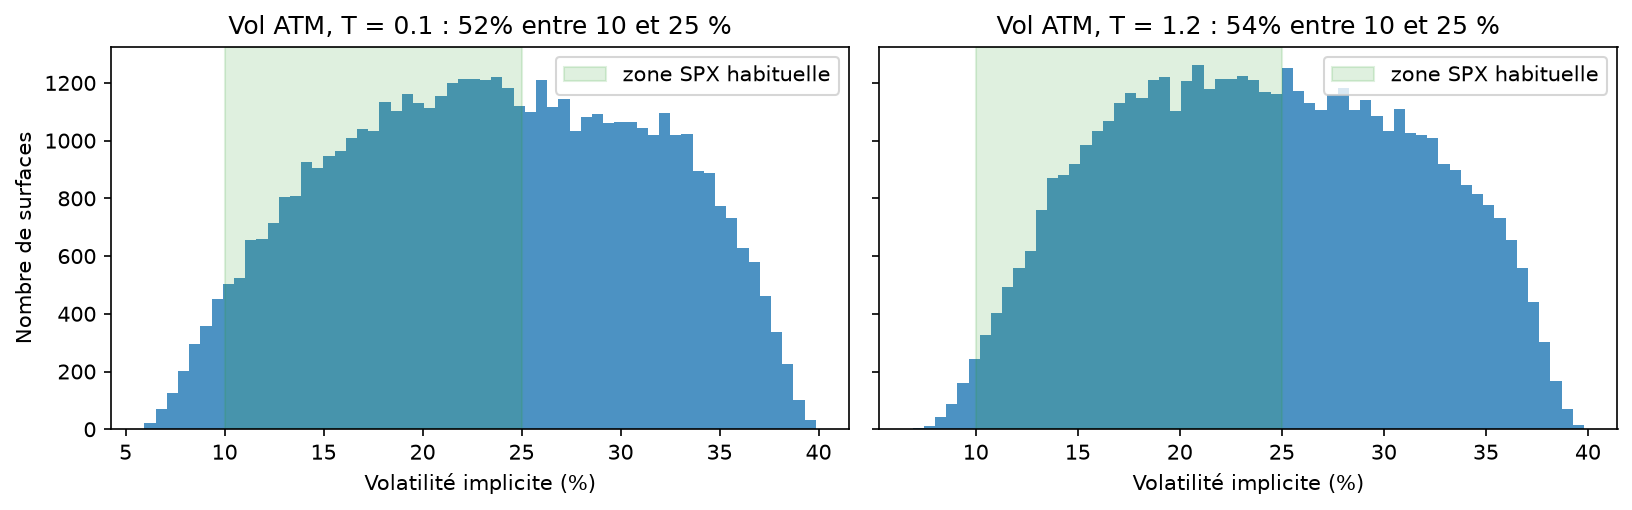
\includegraphics[width=\textwidth]{etape0_vols_atm}
  \caption{Répartition de la volatilité implicite à la monnaie ($K=1$) dans le jeu d'entraînement, à 1 mois et à
  1,2 an. La bande verte est la zone habituelle du SPX.}
  \label{fig-vols-atm}
\end{figure}

\subsection{Le jeu d'entraînement}
\label{sec-jeu}

Nous avons généré \num{50000} surfaces (\texttt{julia/generate\_data.jl}, graine \num{42}), découpées en
\num{40000} pour l'entraînement, \num{5000} pour la validation et \num{5000} pour le test (\SI{80}{\percent} /
\SI{10}{\percent} / \SI{10}{\percent}). Les paramètres sont tirés avant le calcul parallèle : le fichier est
identique quel que soit le nombre de threads. La \cref{fig-surfaces} montre quatre surfaces tirées au hasard : on
retrouve le skew négatif ($\rho<0$), qui s'aplatit quand la maturité augmente.

\begin{figure}[H]
  \centering
  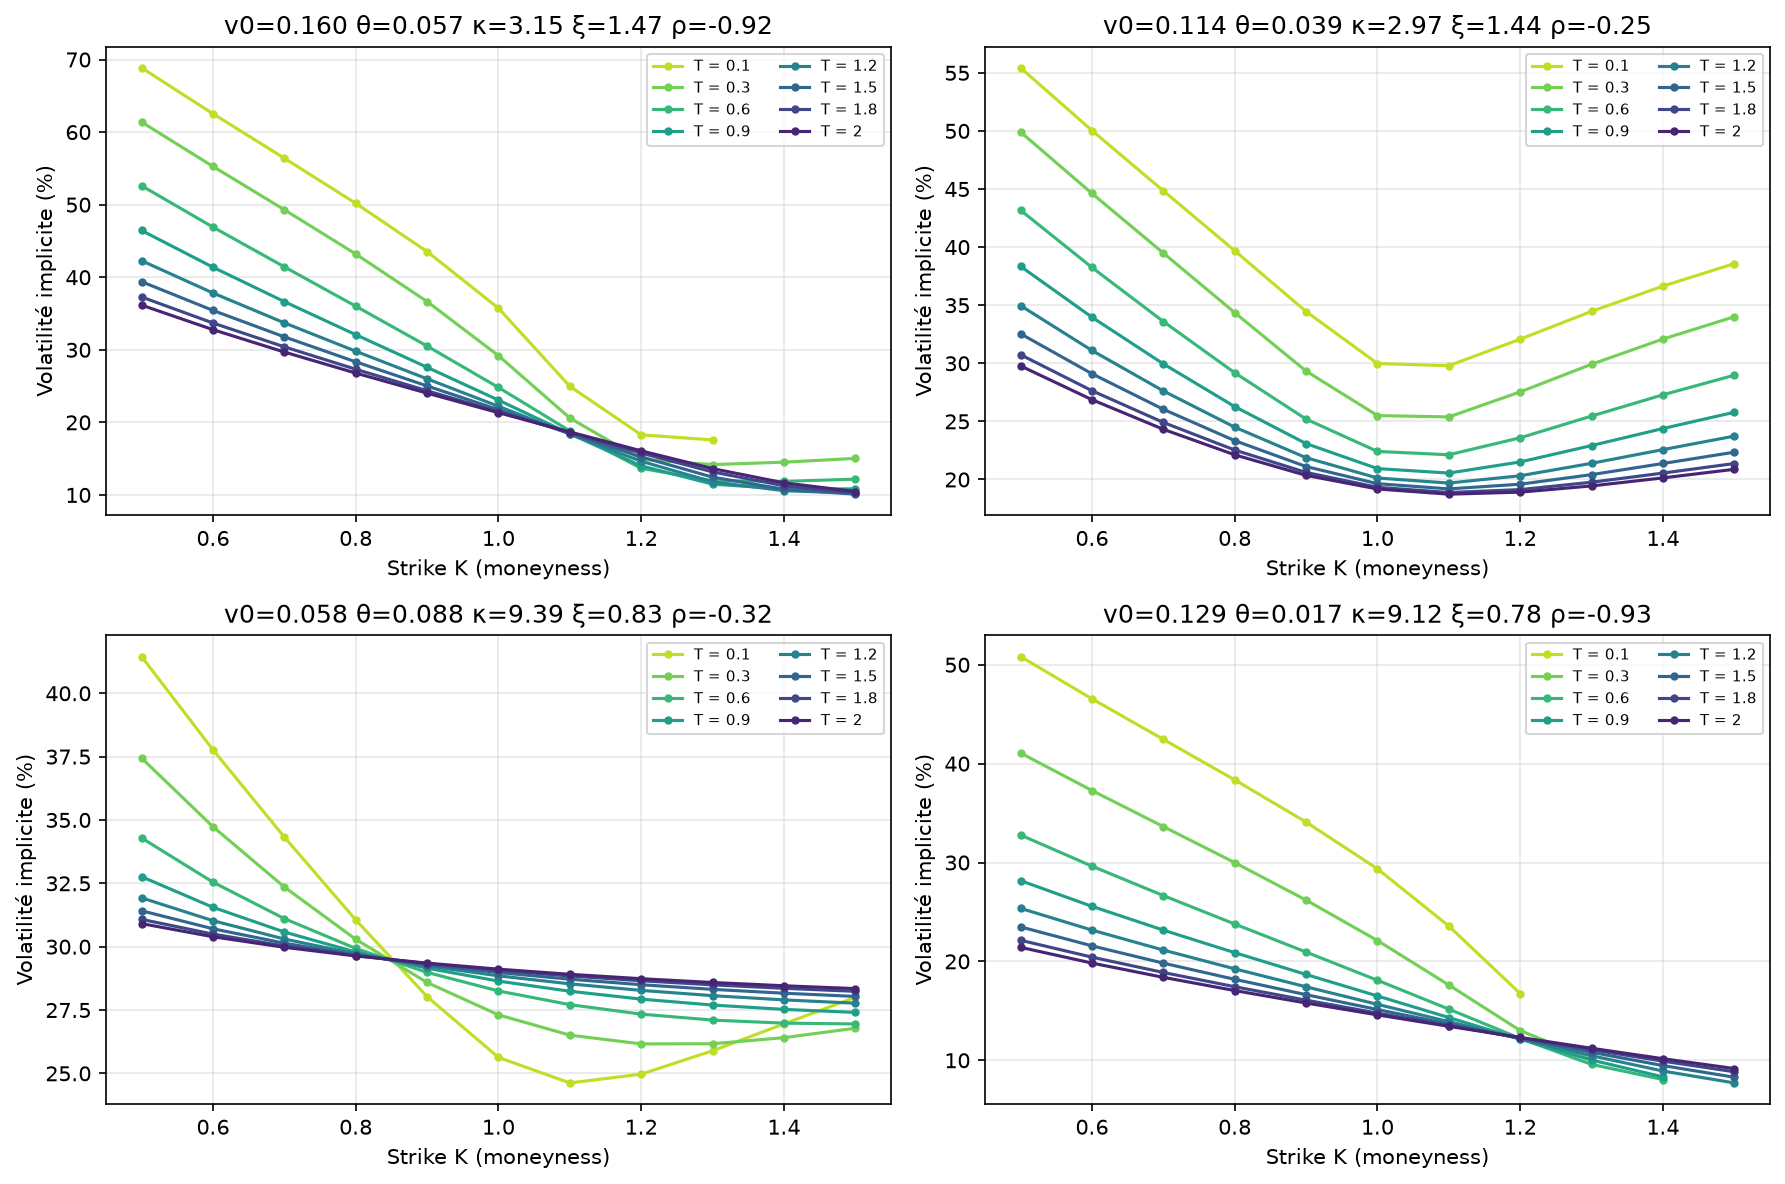
\includegraphics[width=\textwidth]{etape0_surfaces}
  \caption{Quatre surfaces du jeu d'entraînement, une courbe par maturité.}
  \label{fig-surfaces}
\end{figure}

\paragraph{Les points manquants.} Une option dont le prix est inférieur à $10^{-10}$ n'a pas de volatilité implicite
fiable : le point est marqué NaN. \SI{56.2}{\percent} des surfaces ont au moins un point manquant, mais cela ne
représente que \SI{1.9}{\percent} des points (\num{83827} sur \num{4400000}). Ils sont presque tous à la maturité
d'un mois, sur les strikes extrêmes (\cref{fig-nan}) : \SI{34}{\percent} des surfaces à $K=0{,}5$, \SI{44}{\percent}
à $K=1{,}5$. Au-delà d'un mois, il ne reste que \SI{0.34}{\percent} de points manquants. Ces options ne sont de
toute façon pas cotées sur le marché. Nous gardons ces surfaces : la perte du réseau et les métriques ignorent
simplement les points manquants. Jeter les surfaces entières ferait perdre plus de la moitié du jeu.

\begin{figure}[H]
  \centering
  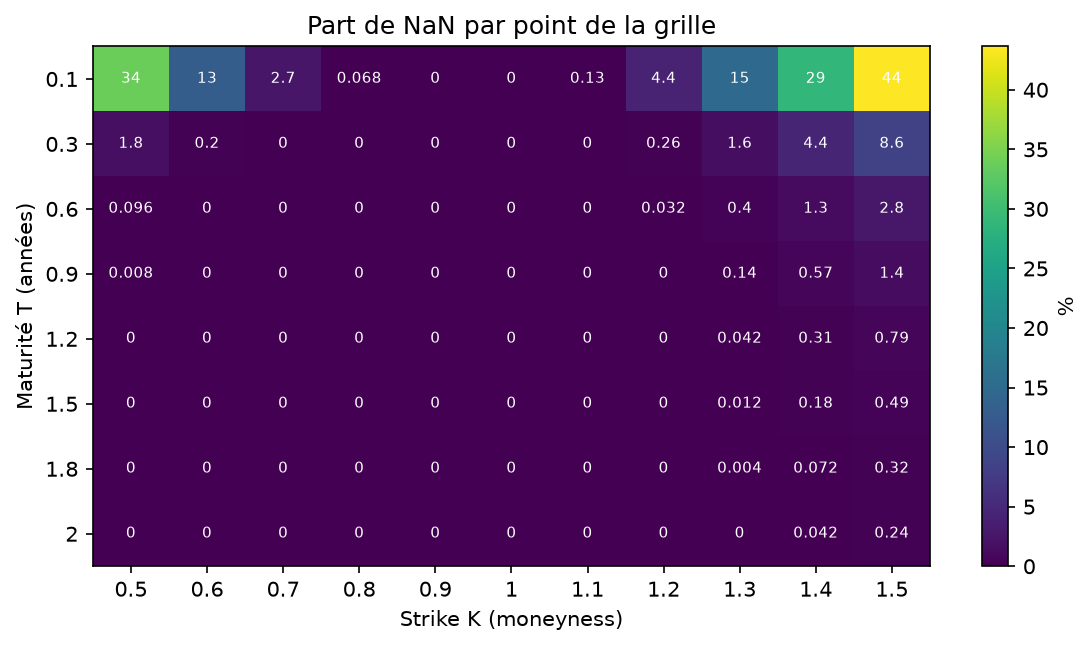
\includegraphics[width=0.85\textwidth]{etape0_nan}
  \caption{Part des surfaces où le point est manquant (NaN), en \%, pour chaque point de la grille.}
  \label{fig-nan}
\end{figure}

\subsection{Le coût de Fourier}
\label{sec-cout}

Le temps de référence que le réseau devra battre est celui d'une surface sur un seul cœur, inversion de
Black-76 comprise. Julia et Python sont mesurés de la même façon, sur les mêmes 200 jeux de paramètres (les 200
premières surfaces du jeu) : pour chaque jeu, un appel à blanc puis cinq mesures dont on garde la médiane ; le
temps retenu est la médiane sur les 200 jeux. Le \cref{tab-temps} compare les deux : Julia est cinq fois plus
rapide sur une surface et presque quatre fois plus rapide sur la génération complète, ce qui justifie de l'avoir
choisi pour la génération des données. Le temps d'une surface dépend beaucoup des paramètres (de \SI{0.9}{\ms} à
\SI{25}{\ms} en Julia), car le nombre de termes de la série COS nécessaire varie, d'où le choix de la médiane.

Ces mesures sont sensibles à la charge de la machine : mesurés pendant que d'autres calculs tournaient, les mêmes
codes prenaient deux à trois fois plus de temps. Tous les temps du projet sont donc mesurés machine au repos, sur
la même machine.

\begin{table}[H]
  \centering
  \caption{Temps de calcul (processeur AMD Zen 5, 20 threads).}
  \label{tab-temps}
  \begin{tabular}{lrrr}
    \toprule
    & Julia & Python & Python / Julia \\
    \midrule
    Une surface, un cœur (médiane)                   & \SI{2.29}{\ms}  & \SI{11.0}{\ms} & \num{4.8} \\
    Génération des \num{50000} surfaces (20 threads) & \SI{23.9}{\s}   & \SI{89.1}{\s}  & \num{3.7} \\
    \bottomrule
  \end{tabular}
\end{table}

Le pricer est réglé pour la précision plutôt que pour la vitesse. Un intervalle de troncature adapté au ratio de
Feller le rendrait environ \SI{30}{\percent} plus rapide, sans changer l'ordre de grandeur du gain du réseau.

\subsection{Les surfaces de marché (SPX)}
\label{sec-spx}

Pour l'étape de calibration, nous avons construit des surfaces réelles à partir des options sur l'indice S\&P 500
(SPX), des options européennes. Les cotations viennent de Yahoo Finance, téléchargées avec la bibliothèque
\texttt{yfinance} pendant les heures d'ouverture américaines. Le traitement (\texttt{src/heston\_nn/data/market.py})
suit les étapes suivantes :
\begin{enumerate}
  \item Nettoyage. On garde les échéances de 7 jours à 2,6 ans et les cotations dont le prix moyen
  (milieu de la fourchette achat-vente) dépasse \num{0.05} et dont la fourchette relative est inférieure à
  \SI{50}{\percent}.
  \item Forward et actualisation. La parité call-put $C - P = D\,(F - K)$ est une droite en $K$. Estimé
  échéance par échéance, le facteur d'actualisation $D$ est très bruité : le 20 novembre, les taux implicites
  allaient de \SI{-36}{\percent} à \SI{235}{\percent}, et une échéance mal estimée décalait toute une ligne de la
  surface d'environ un point de volatilité. Nous estimons donc \emph{un seul taux par jour} (médiane des échéances
  d'au moins trois mois), en déduisons $D = e^{-rT}$ pour toutes les échéances, puis le forward de chacune par
  $F = K + (C-P)/D$ sur les strikes proches de la monnaie.
  \item Volatilités implicites des options hors de la monnaie, par la formule de Black-76.
  \item Lissage. Pour chaque échéance, un smile SVI \citep{gatheral2014} est ajusté sur les strikes
  $K/F \in [0{,}4 ; 1{,}7]$.
  \item Projection sur la grille, par interpolation linéaire de la variance totale $\sigma^2 T$ entre les
  échéances. Un masque indique les points réellement couverts par des cotations ; les autres sont extrapolés
  par les smiles SVI.
\end{enumerate}

\paragraph{Précision de la chaîne.} Nous l'avons testée sur une chaîne d'options fictive générée par Heston, avec un
taux, un dividende et une fourchette achat-vente de $\pm\SI{1}{\percent}$ (\texttt{tests/test\_market.py}). Le
taux et le forward sont retrouvés exactement, et la surface reconstruite est à \SI{8}{\pb} en moyenne de la vraie,
\SI{35}{\pb} au maximum, aux maturités courtes. Cet écart vient du lissage SVI, qui ne peut pas reproduire
exactement un smile de Heston. C'est l'ordre de grandeur de la précision qu'on peut attendre d'une surface de
marché ; il faudra s'en souvenir en lisant les erreurs de calibration.

\paragraph{Les jours collectés.} Yahoo Finance ne donne que les cotations du moment, sans historique : chaque jour
doit être téléchargé le jour même, et le fichier brut est conservé (\texttt{data/spx/raw/}) pour pouvoir
reconstruire la surface. Le \cref{tab-spx-jours} résume les quatre jours disponibles. Le marché a baissé
d'environ \SI{7}{\percent} entre le 4 et le 20 novembre, et la volatilité à un mois est passée de
\SI{13.4}{\percent} à \SI{22.5}{\percent}. Les quelques violations d'arbitrage calendaire (variance totale qui
diminue avec la maturité) sont presque toutes dans l'aile des calls ($K \geq 1{,}3$), hors de la zone de
calibration.

\begin{table}[H]
  \centering
  \caption{Surfaces SPX collectées. « Coté » : part de la grille couverte par des cotations ;
  « Viol. » : violations d'arbitrage calendaire.}
  \label{tab-spx-jours}
  \begin{tabular}{lrrrrrr}
    \toprule
    Date & Spot & Taux & Échéances & Coté & Viol. & Vol ATM 1 mois \\
    \midrule
    3 nov.\ 2026  & \num{7569} & \SI{4.85}{\percent} & 44 & \SI{83}{\percent} & 7 & \SI{16.0}{\percent} \\
    4 nov.\ 2026  & \num{7689} & \SI{4.84}{\percent} & 43 & \SI{82}{\percent} & 7 & \SI{13.4}{\percent} \\
    5 nov.\ 2026  & \num{7422} & \SI{4.90}{\percent} & 42 & \SI{83}{\percent} & 7 & \SI{19.6}{\percent} \\
    20 nov.\ 2026 & \num{7140} & \SI{5.85}{\percent} & 42 & \SI{88}{\percent} & 4 & \SI{22.5}{\percent} \\
    \bottomrule
  \end{tabular}
\end{table}

Le taux du 20 novembre est moins sûr que les autres : les estimations par échéance étaient beaucoup plus
dispersées (de \SI{3.4}{\percent} à \SI{9.6}{\percent} entre le premier et le dernier quartile, contre
\SIrange{4.7}{5.0}{\percent} le 4 novembre), probablement parce que les cotations ont été téléchargées juste après
l'ouverture.

\begin{figure}[H]
  \centering
  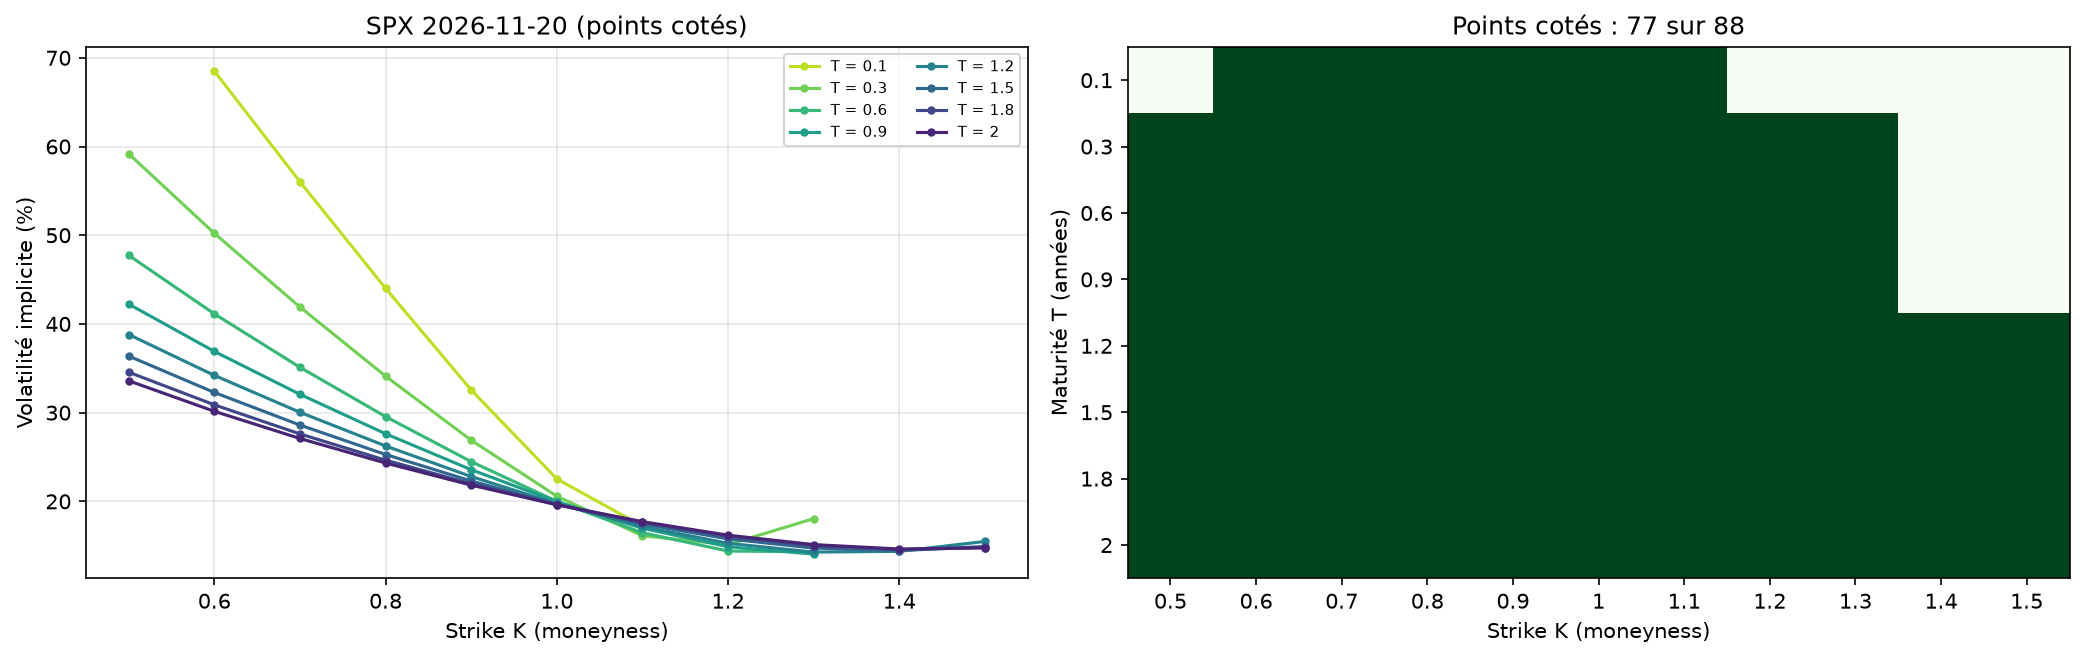
\includegraphics[width=\textwidth]{etape0_spx}
  \caption{Surface SPX du dernier jour collecté (points cotés seulement) et masque des points cotés.}
  \label{fig-spx}
\end{figure}

\paragraph{La zone de calibration.} Le skew du SPX à court terme est extrêmement raide : le 4 novembre, à un mois,
la volatilité valait \SI{13.4}{\percent} à la monnaie mais \SI{71.7}{\percent} pour $K = 0{,}5$. Le modèle de
Heston, sans sauts, ne peut pas produire une telle pente sur une maturité aussi courte. C'est une limite connue,
qui motive notamment les modèles à volatilité rugueuse étudiés par \citet{horvath2021}. Calibré sur tous les points
cotés, Heston fait de \SI{100}{\pb} à \SI{170}{\pb} d'erreur moyenne selon les jours, jusqu'à 20 points de
volatilité sur certains points, et ses paramètres partent vers des valeurs extrêmes (sans borne, $\xi \approx 4$ à 5
et un ratio de Feller proche de \num{0.05}). Nous calibrons donc sur la zone liquide,
proche de la monnaie : strikes de \num{0.7} à \num{1.3} et maturités d'au moins \num{0.3} an (49 points de la grille,
réglage \texttt{spx\_calibration} de \texttt{base.yaml}). Les autres points restent dans les données mais ne servent
pas à calibrer.

\paragraph{Calibration d'essai.} Avant l'étape~4, nous avons calibré les quatre jours avec le pricer Fourier et le
même optimiseur que l'étape~4 (Levenberg-Marquardt, cinq points de départ), sur cette zone
(\cref{tab-spx-calibration}, \cref{fig-spx-calibration}).

\begin{table}[H]
  \centering
  \caption{Calibration de Heston sur les surfaces SPX (pricer Fourier, zone de calibration). Erreurs en points de
  base ; « tous » : erreur moyenne sur tous les points cotés, pour comparaison.}
  \label{tab-spx-calibration}
  \begin{tabular}{lrrrrrrrr}
    \toprule
    Date & $v_0$ & $\theta$ & $\kappa$ & $\xi$ & $\rho$ & Feller & Zone (moy.~/ max) & Tous \\
    \midrule
    3 nov.  & \num{0.036} & \num{0.049} & \num{3.89} & \num{1.5} & \num{-0.72} & \num{0.17} & \num{29.2} / 146 & 98 \\
    4 nov.  & \num{0.023} & \num{0.049} & \num{3.99} & \num{1.5} & \num{-0.71} & \num{0.17} & \num{29.5} / 125 & 120 \\
    5 nov.  & \num{0.053} & \num{0.050} & \num{3.82} & \num{1.5} & \num{-0.75} & \num{0.17} & \num{29.1} / 165 & 141 \\
    20 nov. & \num{0.076} & \num{0.055} & \num{3.89} & \num{1.5} & \num{-0.76} & \num{0.19} & \num{29.8} / 123 & 94 \\
    \bottomrule
  \end{tabular}
\end{table}

Les paramètres sont stables d'un jour à l'autre ($\kappa \approx 3{,}9$, $\theta \approx 0{,}05$,
$\rho \approx -0{,}73$), et $v_0$ suit la volatilité de court terme du marché. Tous restent dans le domaine
d'entraînement (ratio de Feller entre \num{0.17} et \num{0.19}), à une exception près : $\xi$ atteint sa borne de
\num{1.5} les quatre jours. Sans borne, il vaudrait environ 2, pour la même erreur moyenne. Élargir le domaine à
$\xi \leq 2{,}5$ ne rendrait pas les grandes zones utilisables (l'obstacle est la maturité d'un mois) et pousserait
le ratio de Feller vers \num{0.1}, au bord du domaine appris : nous avons gardé $\xi \leq 1{,}5$.

\begin{figure}[H]
  \centering
  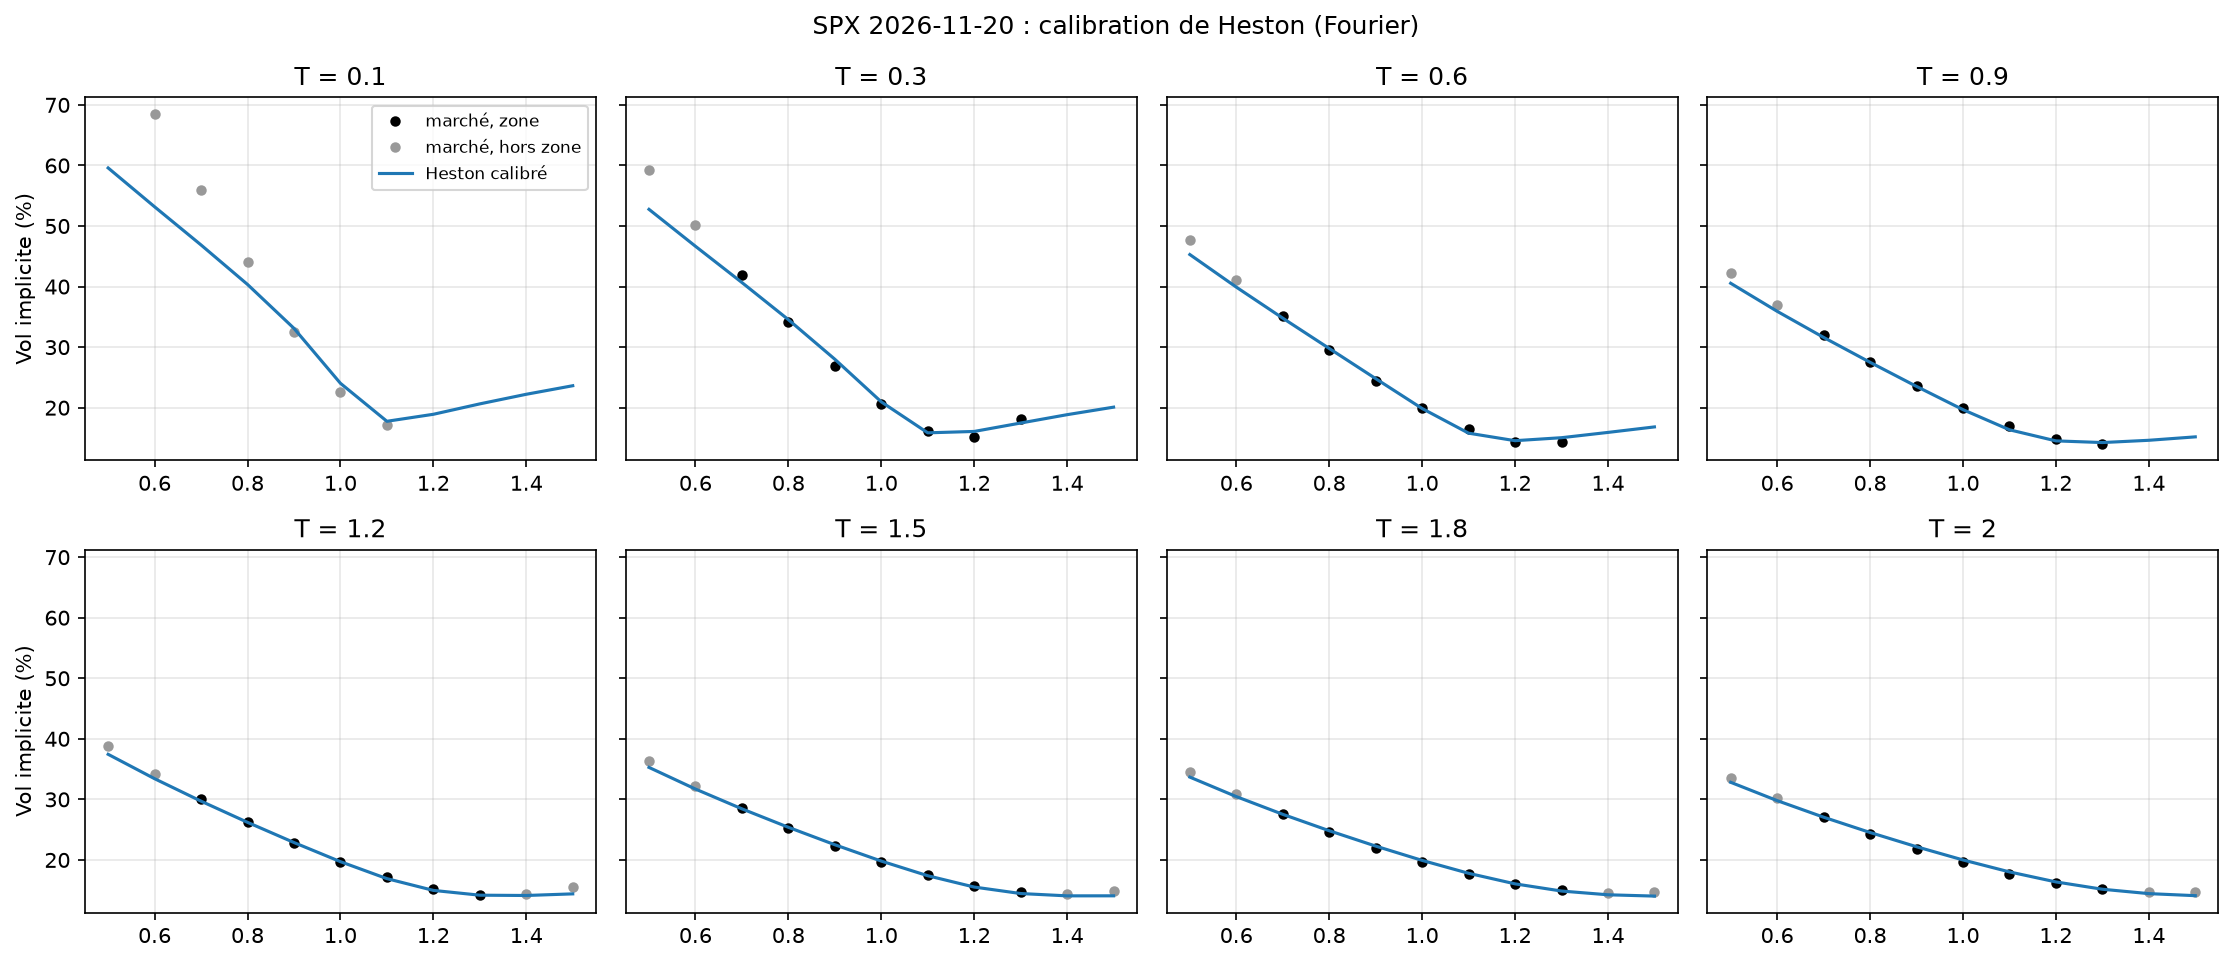
\includegraphics[width=\textwidth]{etape0_spx_calibration}
  \caption{Calibration du 20 novembre, maturité par maturité : points du marché dans la zone (noirs) et hors zone
  (gris), et Heston calibré (trait).}
  \label{fig-spx-calibration}
\end{figure}

\subsection{Limites}
\label{sec-limites-donnees}

\begin{itemize}
  \item Nous avons peu de jours de marché, tous dans le même régime. Yahoo Finance ne fournit pas d'historique :
  nos surfaces SPX couvrent quelques jours de novembre 2026, avec une volatilité entre \SI{13}{\percent} et
  \SI{23}{\percent}. Elles montrent la calibration sur données réelles, mais ne disent rien d'un marché très calme
  ou en crise. Il faudrait pour cela une base historique (OptionMetrics, par exemple).
  \item La surface de marché a sa propre imprécision, due au lissage SVI : environ \SI{8}{\pb} en moyenne sur des
  données fictives, plus avec le bruit réel. C'est du même ordre que l'erreur du réseau.
  \item Sur le SPX, $\xi$ atteint sa borne, et Heston ne peut pas reproduire le skew à un mois : nous calibrons
  sur une zone réduite de la surface.
\end{itemize}
